\documentclass{beamer}
\usetheme{Szeged}
%To define color
\definecolor{mycolor}{rgb}{.125,170.125,0.125} % color
\usecolortheme{crane}

    
\includegraphics[width=0.6\textwidth]{uh.PNG}

    % 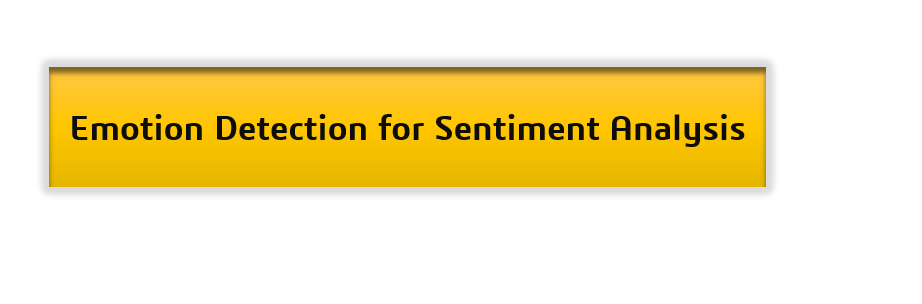
\includegraphics[width=1.0\textwidth]{Emotionhead.PNG}
      \title{Emotion Detection for Sentiment Analysis} 
      
    \author {\color{red} \item Mamatha Vantipenta-17056721  \item Brijrajsinh Ranjitsinh Gohil -17062221  \item Madhav Reddy Ramasani -17061360  \item Nusrat Alam Moni -17066047}
   

\begin{document}
\begin{frame}
    \titlepage
\end{frame}
% Slide 1
\begin{frame}{Agenda}
\begin{enumerate}\vspace{12pt}
    \item Overview of the Project 
    \item What is Emotion Detection and how it carries?
    \item Graphical User Interface
    \item Related Tests and Training
    \item Confusion Matrix
    \item Technologies Used
       \item Thank You
\end{enumerate}
\end{frame}
%Slide 2
\begin{frame}{Overview of the Project}\vspace{1pt}
\begin{enumerate}
\pagenumbering{roman}
\item The main aim of the project is to improve Graphical user interface and adding the new features to redevelop an existing system. 
\item The project will attempt to determine if there is a significant difference in performance before and after adding the features.
\item It also aims to make the GUI more user friendly.
\item The project aims to prove that there is no significant change in the winning algorithm.
\end{enumerate}
\end{frame}
%Slide 3
\begin{frame}{What is Emotion Detection and how it carries?}
\begin {enumerate}
\item Nowadays the use of advance technology and internet becomes an essential part of human beings.Since last two decades the use of technology and internet for the purpose of entertainment and it is getting increased day by day.\item "Emotions can be defined as a positive or negative experience that is associated with a particular pattern of physiological activity."Emotions produce different physiological, behavioral and cognitive changes.\item Emotion recognition is a method used in software that permits a program to “examine” the sentiments on a human face by utilizing sophisticated image dispensation.
\end {enumerate}
    \centering
    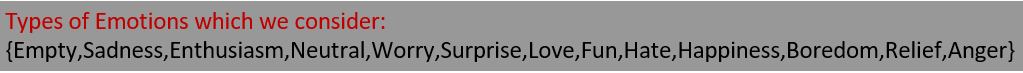
\includegraphics[width=0.9\textwidth]{Emotions.PNG}
           
\end{frame}
%Slide 4
\begin{frame}{Graphical User Interface}
\centering
    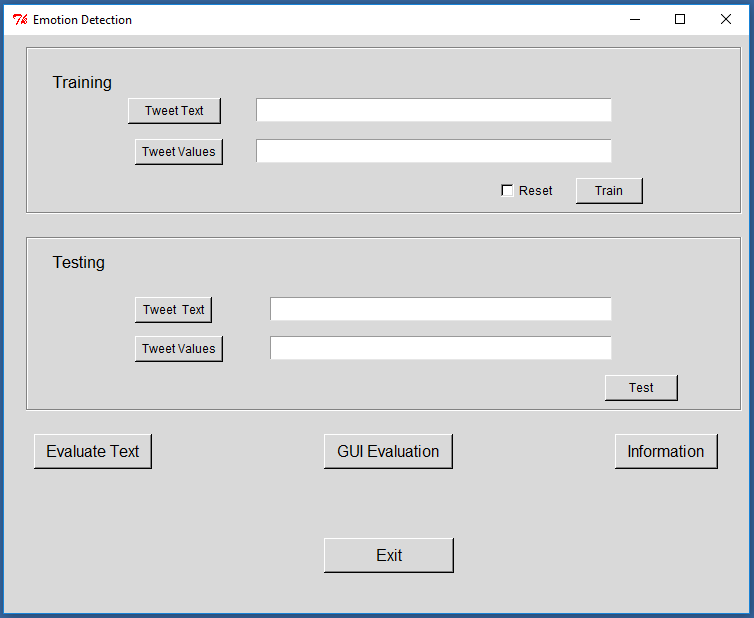
\includegraphics[width=0.8\textwidth]{Overview.png}
\end {frame}
%Slide 5
\begin{frame}{Graphical User Interface Contd..}
\centering
    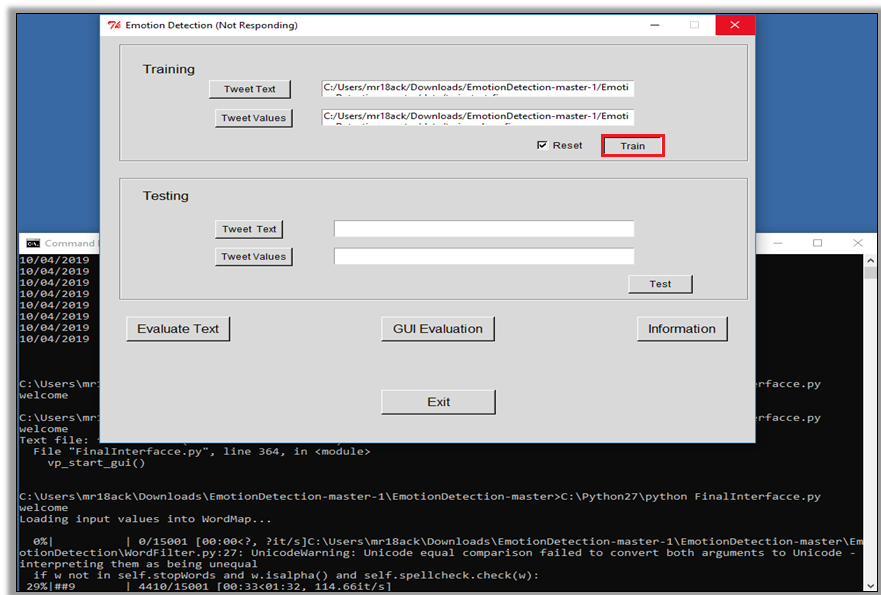
\includegraphics[width=0.9\textwidth]{Training.png}
\end {frame}
%Slide 6
\begin{frame}{Graphical User Interface Contd..}
\centering
    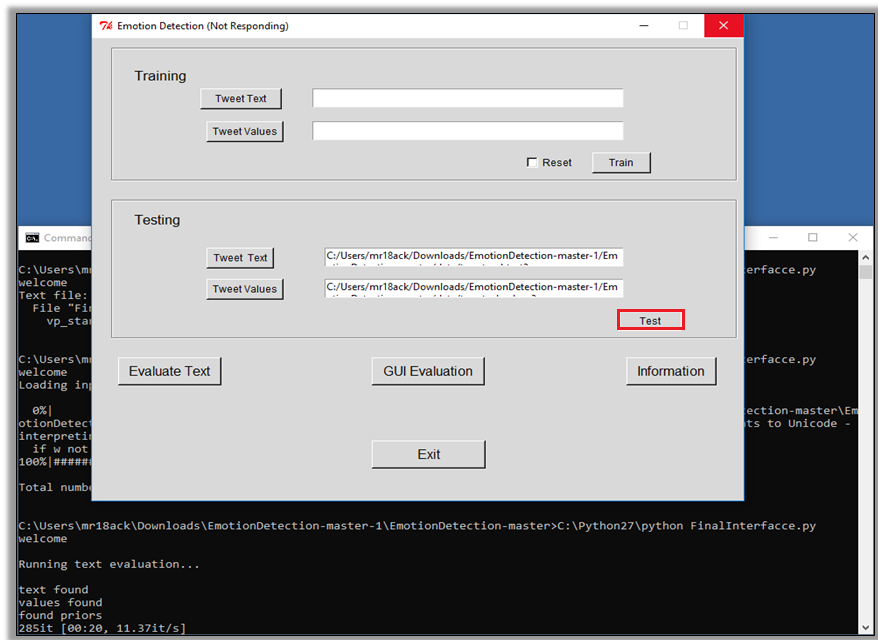
\includegraphics[width=0.9\textwidth]{Test.png}
\end {frame}
%Slide 7
\begin{frame}{Graphical User Interface Contd..}
\centering
    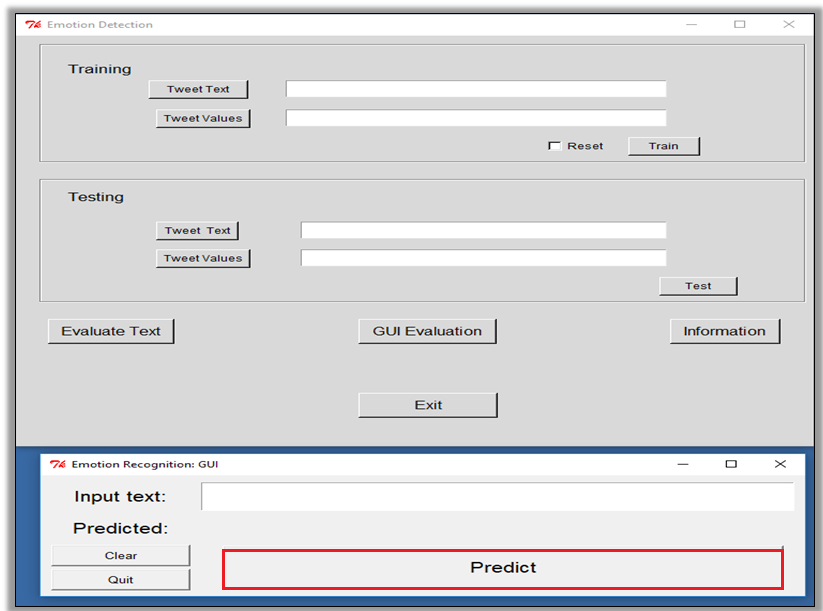
\includegraphics[width=0.9\textwidth]{Predict.png}
\end {frame}
%Slide 8
\begin {frame}{Related Tests and Training}
\begin {enumerate}
\item Training: Generates a Word Map using a text file and emotion value file.A word map is required for both testing and evaluation.\item Testing:Run the system and test its accuracy by supplying emotion values it also produces reports and confusion plot.
    \beginleft
    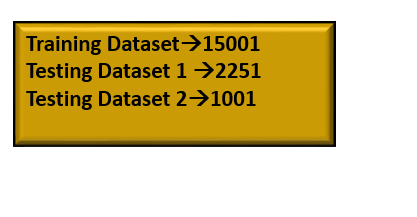
\includegraphics[width=0.8\textwidth]{Values.PNG}
    \endleft
   \end {enumerate}
\end {frame}
%slide 9
\begin {frame}{Related Tests and Training Contd..}
    \centering
    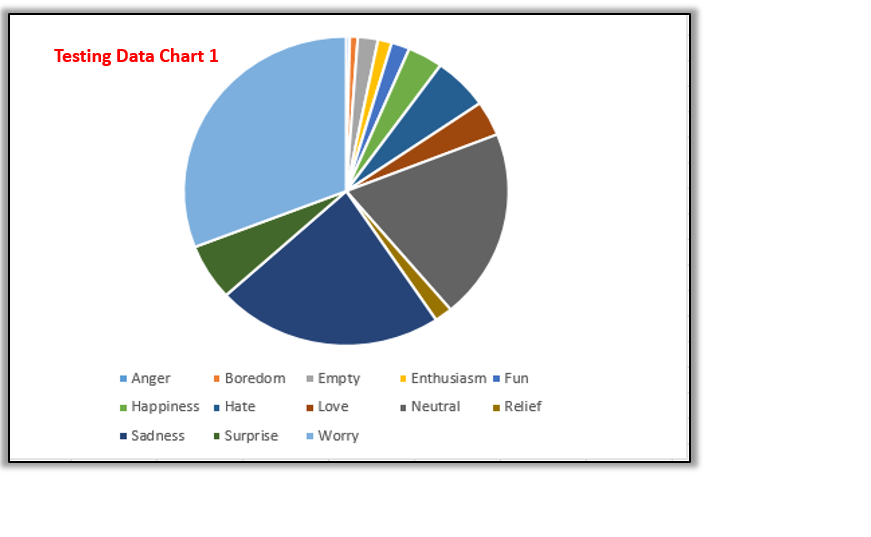
\includegraphics[width=1.0\textwidth]{2251.PNG}
    \end {frame}
    %slide 10
 \begin {frame}{Related Tests and Training Contd..}
 \centering
        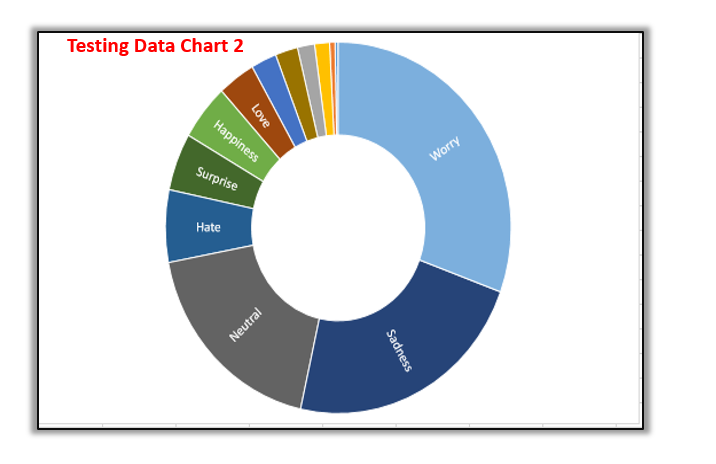
\includegraphics[width=0.9\textwidth]{10001.PNG}
    \endleft
   \end {frame}


%Slide 11
\begin{frame}{Confusion Matrix 1}
\centering
    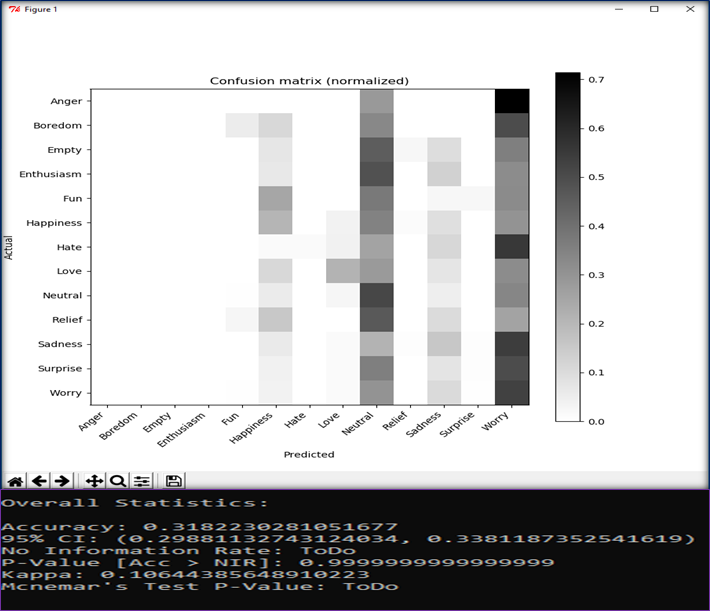
\includegraphics[width=0.8\textwidth]{Confusion1.png}
  
\end{frame}
%Slide 12
\begin{frame}{Confusion Matrix 2}
     \centering
    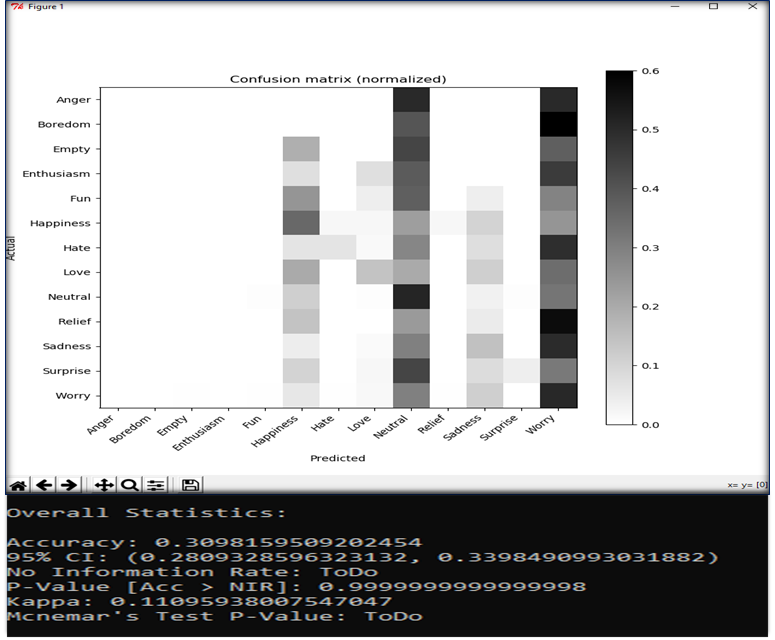
\includegraphics[width=0.8\textwidth]{Confusion2.png}
    \caption{}
    \end{frame}
   %Slide 12
\begin{frame}{Technologies Used}
     \beginleft
     \begin{enumerate}
     \begin{itemize}
         \item Python 2.7
         \item LATEX
    \item MS Excel
    \item GIT and Git Hub
     \end{itemize}
        \end{enumerate}
       \endleft
     \end{frame} 
%Slide 13
\begin{frame}
\centering

\includegraphics[width=1.0\textwidth]{Thank.png}
\end {frame}
\end{document}